% Chapter 3
\chapter{Análise e discussão de resultados}\label{chap:Results}

Ao decorrer deste capítulo são apresentados, respectivamente, a identificação das partes interessadas no aplicativo seguido de suas necessidades e problemas, a análise do sistema com os diagramas de processo, caso de uso e diagramas de classe. Em seguida é apresentada a proposta de aplicativo, o protótipo, os resultados esperados e as áreas que serão afetadas pelo app.

\section{Situação Atual}
O aplicativo será desenvolvido baseado no ambiente da empresa Abase Sistemas e Soluções LTDA, uma empresa de software localizada na cidade de Três de Maio - RS e com sua fundação realizada em 1989. Atualmente a Abase tem duas áreas de trabalho bem definidas. Uma das áreas desenvolve sistemas para a gestão pública, tendo como clientes a maior parte das prefeituras da região, e a outra área trabalha no desenvolvimento de um ERP para empresas privadas, tendo como objetivo fornecer as melhores inovações tecnológicas através de seus softwares aplicativos integrados. 

Ao conversar com o responsável de infraestrutura da empresa, foi possível observar que atualmente não há controle para os chamados internos de infraestrutura de TI em específico, só há registros dos chamados de requisição de serviços de suporte para desenvolvimento e vice-versa em para chamados de clientes. Quando há necessidade de solicitar algo para a infraestrutura, usa-se telefone, \textit{Skype}, \textit{Whatsapp} ou até mesmo indo pessoalmente até a sala do responsável e descrevendo o problema. Ou seja, não há uma forma padrão para criar ou responder chamados, o que de acaba prejudicando o gerenciamento de processos.

Os chamados que são registrados, são feitos através do sistema de atendimento ao cliente de uma empresa terceirizada tendo a empresa cadastrada como um cliente e os funcionários como usuários. O grande problema sempre ao ter um sistema para gerenciar os chamados é convencer o usuário a usar, para adotar o uso se faz necessário exigir o cadastro de uma tarefa no sistema de chamados para a mesma ser executada. Caso seja exigida a execução de um serviço, o mesmo não poderia ser feito sem ter um chamado associado. 

De acordo com as próprias palavras do responsável, o fato de ter um aplicativo como o proposto, poderia permitir que um chamado fosse fechado assim que uma tarefa foi executada, em qualquer lugar. Por exemplo; ao trocar o teclado de um usuário que já havia feito o pedido, o responsável pela troca poderia finalizar o chamado no local, sem ter a necessidade de retornar ao seu computador para faze-lo.

\section{Especificação dos requisitos e processos}
% Deve descrever o que se deseja do sistema a ser desenvolvido. Não são necessários  modelos gráficos neste item. Os principais subitens da especificação são:
Ao dispor a contextualização da situação atual do processo na empresa e também dos objetivos e problema propostos, é possível escalar as funcionalidades que se desejam no aplicativo. 

O app está sendo desenvolvido tendo como foco padronizar a forma de gerar chamados de suporte de TI internamente na empresa. Em geral, o aplicativo deve permitir a abertura de chamados, o monitoramento de chamados abertos, fechar chamados, classificar um chamado como pausado, classificar um chamado como aberto, finalizar chamado aberto e também permitir a visualização dos detalhes de um chamado independente do status.


\subsection{Requisitos funcionais} %casos de uso e funcionalidades
Como requisitos funcionais podem ser identificados os casos de: criar chamado, atender chamado, pausar chamado,  retomar atendimento de chamado pausado, finalizar chamado e ver detalhes de chamado. Os requisitos funcionais são descrições específicas dos casos de uso que são aplicados as regras de negócio, conforme o diagrama de caso de uso, ilustrado na Figura \ref{fig:diagrama_caso_de_uso}.

\begin{figure}[htb]
     \caption{Diagrama de caso de uso}
     \centering
     \begin{frame}{
     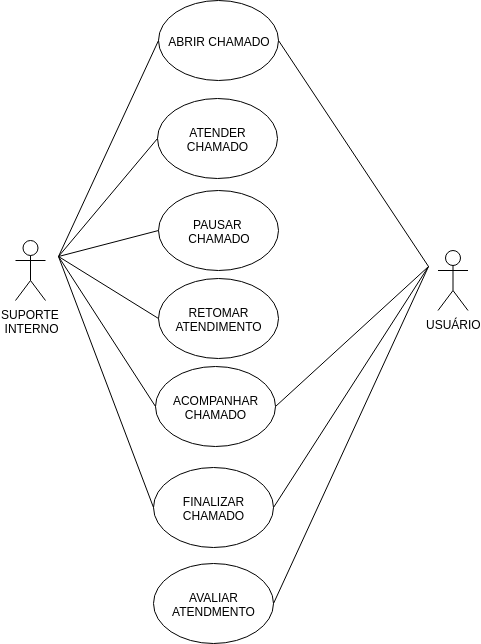
\includegraphics [scale = 0.7]{img/Diagramas/diagrama_caso_de_uso.png}}
     \end{frame}
     \label{fig:diagrama_caso_de_uso}
 \end{figure}
\newpage
Portanto, a partir da ilustração do diagrama, é possível identificar os requisitos funcionais do aplicativo para  então descrever os mesmos. Os requisitos identificados são Criar Chamado, Atender chamado, pausar chamado, retomar atendimento, finalizar chamado e avaliar atendimento, os quais estão respectivamente descritos como:\\

\noindent\fbox{
    \parbox{\textwidth}{
        \small\textbf{RF1 - Criar Chamado} \smallskip\hrule\ \\
        \small\textbf{Descrição:} A criação de um chamado é o início do fluxo do chamado no sistema. Após o chamado ser criado, o mesmo entra em \textit{workflow} onde é possível visualizar o status do chamado conforme o andamento do mesmo e então interagir com os cartões de chamado.\\
        \small\textbf{Ator:} Atendente ou Usuário.\\
        \small\textbf{Entrada:} É necessário informar um título, a classificação e a descrição do incidente, podendo também anexar uma imagem. A classificação pode ser Hardware, software, rede, impressora, ou telefonia. Além da classificação o usuário deve informar o tipo do chamado, que pode ser Incidente, Requisição de Serviço ou Melhoria.\\ 
        \small\textbf{Saída Principal:} após clicar no botão de concluir, exibir uma mensagem de confirmação.\\
        \small\textbf{Saída alternativa:} caso campos obrigatórios não sejam preenchidos, notificar nos campos através dos validadores.
        \\
    }
}

\noindent\fbox{
	    \parbox{\textwidth}{
	        \small\textbf{RF2 - Atender Chamado} \smallskip\hrule\ \\
	        \small\smallskip\textbf{Descrição:} Para iniciar o atendimento, o chamado já \smalldeve ter sido criado anteriormente e deve estar com status "em espera". Essa função tem como objetivo destacar o chamado como estando em atendimento. \\
	        \small\textbf{Ator:} Atendente. \\
	        \small\textbf{Entrada:} Como entrada pode ser considerado o chamado em si e também a confirmação no botão de atender, inserido no cartão do chamado\\
	        \small\textbf{Saída Principal:} O cartão do chamado deve ir para aba "em atendimento".\\
	    }
	}

\noindent\fbox{
	    \parbox{\textwidth}{
	        \small\textbf{RF3 - Priorizar Chamado} \smallskip\hrule\ \\
	        \small\smallskip\textbf{Descrição:} Ao atender um chamado, o atendente deve classificar o mesmo em relação a seu nível de prioridade. \\
	        \small\textbf{Ator:} Atendente. \\
	        \small\textbf{Entrada:}O chamado deve ser classificado de acordo com sua prioridade, podendo ser Baixo, Médio, Alto ou Crítico.\\
	        \small\textbf{Saída Principal:} O cartão do chamado deve apresentar um ícone identificador para cada uma destas situações.\\
	    }
	}
	
\noindent\fbox{
	    \parbox{\textwidth}{
	        \small\textbf{RF4 - Ordenar Lista de Chamados} \smallskip\hrule\ \\
	        \small\smallskip\textbf{Descrição:} Ordena a lista de chamados de acordo com sua prioridade ou data de abertura do chamado. \\
	        \small\textbf{Ator:} Atendente ou Usuário. \\
	        \small\textbf{Entrada:}Como entrada pode ser considerado o filtro utilizado.\\
	        \small\textbf{Saída Principal:} Deve retornar a listagem seguindo o ordenamento definido pelo Atendente ou Usuário.\\
	    }
	}

\noindent\fbox{
	    \parbox{\textwidth}{
	        \small\textbf{RF5 - Pausar Chamado} \smallskip\hrule\ \\
	        \small\smallskip\textbf{Descrição:} A função de pausar chamado refere-se a necessidade de deixar um chamado pausado depois de já ter sofrido o primeiro atendimento. Um chamado pausado diferencia-se de um chamado em espera pelo fato de que um chamado em espera não passou pelo primeiro atendimento ainda, apenas pela abertura do mesmo.  \\
	        \small\textbf{Ator:} Atendente. \\
	        \small\textbf{Entrada:}Como entrada pode ser considerado o chamado em si e também a confirmação no botão de pausar chamado. \\ 
	        \small\textbf{Saída Principal:} O cartão do chamado deve ir para aba "pausado". \\
	    }
	}

\noindent\fbox{
        \parbox{\textwidth}{
            \small\textbf{RF6 - Retomar Atendimento} \smallskip\hrule\ \\
            \small\textbf{Descrição:} A função de retomar tem por objetivo retomar o atendimento do chamado pausado.  \\
            \small\textbf{Ator:} Atendente \\
            \small\textbf{Entrada:} Como entrada pode ser considerado o chamado em si e também a confirmação no botão de "Retomar Chamado". \\
            \small\textbf{Saída Principal:} O cartão do chamado deve ir para aba "em atendimento".\\
        }
    }
    
\noindent\fbox{
    \parbox{\textwidth}{
        \small\textbf{RF7 - Acompanhar Chamado} \smallskip\hrule\ \\
        \small\textbf{Descrição:} Deve permitir tanto ao usuário quanto ao atendente de suporte visualizar detalhes acerca do chamado, independente do status em que o chamado se encontra.\\
        \small\textbf{Ator:} Atendente ou Usuário\\
        \small\textbf{Entrada:} O usuário/atendente deve selecionar o chamado que desejam consultar. \\
        \small\textbf{Saída Principal:} Exibe detalhes do chamado selecionado.\\
        \small\textbf{Saída alternativa:} Deve informar que os detalhes não puderam ser carregados.\\
    }
}

\noindent\fbox{
        \parbox{\textwidth}{
            \small\textbf{RF8 - Finalizar Chamado} \smallskip\hrule\ \\
            \small\textbf{Descrição:} Permite ao atendente finalizar o chamado, alterando o status para "Concluído".\\
            \small\textbf{Ator:} Atendente\\
            \small\textbf{Entrada:} O atendente deve marcar o chamado como "Concluído".\\
            \small\textbf{Saída Principal:} Informa que o chamado foi concluído com sucesso.\\
        }
    }
    
\noindent\fbox{
        \parbox{\textwidth}{
            \small\textbf{RF9 - Avaliar Atendimento} \smallskip\hrule\ \\
            \small\textbf{Descrição:} O usuário poderá avaliar o atendimento com notas entre 1 e 5 após o encerramento do chamado. Esta avaliação não é obrigatória. \\
            \small\textbf{Ator:} Usuário\\
            \small\textbf{Entrada:} O usuário poderá selecionar um valor entre 1 e 5 ou optar por não responder.\\ 
            \small\textbf{Saída Principal:} Informa que o atendimento foi concluído.\\
        }
    }
    
\noindent\fbox{
        \parbox{\textwidth}{
            \small\textbf{RF10 - Registro de Resolução} \smallskip\hrule\ \\
            \small\textbf{Descrição:} Ao final do atendimento, o atendente poderá registrar o que foi realizado para que a situação fosse resolvida, para que possa consultar caso tenha dúvida em futuros atendimentos. \\
            \small\textbf{Ator:} Atendente\\
            \small\textbf{Entrada:} O atendente poderá informar o que foi realizado para resolver o chamado em questão.\\ 
            \small\textbf{Saída Principal:} Informa que a resposta foi registrada.\\
        }
    }

\subsection{Requisitos não funcionais}
Os requisitos não funcionais são aqueles necessários para o funcionamento da aplicação, porém não interferem nas regras de negócio. De tal forma, foram elencados como requisitos não funcionais foram Sistema operacional Android, Conexão com Internet, Sincronização com banco de dados e Login, respectivamente descritos abaixo:

\noindent\fbox{
    \parbox{\textwidth}{
        \small\textbf{RNF1 - Sistema Operacional Android} \smallskip\hrule\ \\
        Para utilização da aplicação, o usuário deve dispor de um smartphone ou tablet que utilize o sistema operacional Android.
    }
}

\noindent\fbox{
    \parbox{\textwidth}{
        \small\textbf{RNF2 - Conexão com Internet} \smallskip\hrule\ \\
        A Conexão com a internet se faz necessária para sincronizar os dados com o serviço do Firebase. O sistema deve ter implementado um modo \textit{offline first} para gravar chamados ou eventuais mudanças nos chamados no próprio smartphone em caso de falta de conexão com a internet.
    }
}

\noindent\fbox{
    \parbox{\textwidth}{
        \small\textbf{RNF3 - Sincronização com banco de dados} \smallskip\hrule\ \\
        O sistema deve ter implementado um modo \textit{offline first} para gravar chamados ou eventuais mudanças nos chamados no armazenamento do próprio smartphone em caso de falta de conexão com a internet. Ao reconectar o dispositivo, a sincronização com o serviço do Firebase deve ser automática
    }
}

\noindent\fbox{
    \parbox{\textwidth}{
        \small\textbf{RNF4 - Login} \smallskip\hrule\ \\
        O acesso de cada usuário do app deve acontecer a partir de um login e senha único por usuário. \\
        Deve haver dois tipos de usuário, sendo um "Atendente" e outro "Usuário" 
    }
}

\section{Identificação do processo} 
Conforme demonstra a Figura \ref{fig:diagrama_processos}, o processo de atendimento se inicia com a ocorrência de algum tipo de problema para o usuário, o qual abre um chamado de suporte. Neste ponto, é permitido ao atendente do suporte atender ou finalizar este chamado, tendo atendido este chamado, ele pode ser pausado conforme necessário. Após finalização do chamado, o usuário pode optar entre avaliar o atendimento ou não. Caso deseje, poderá dar a sua avaliação através de uma pontuação entre 1 e 5.

\begin{figure}[htb]
     \caption{Diagrama de processo}
     \centering
     \begin{frame}{
         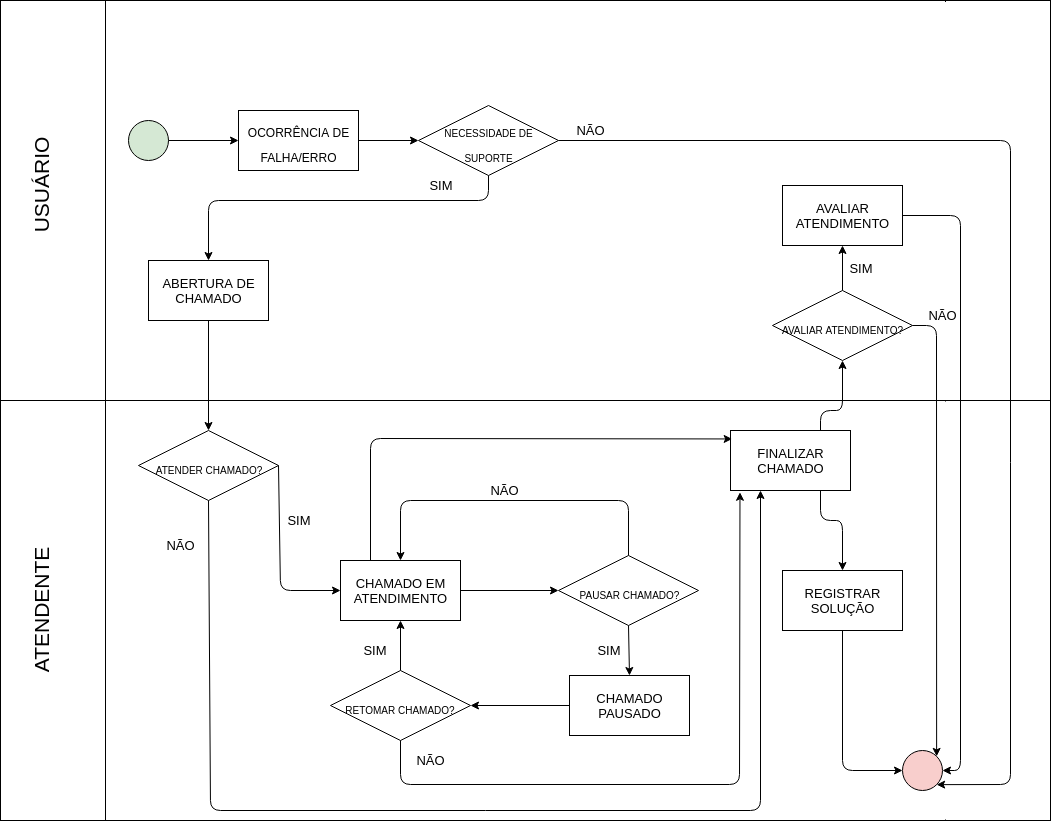
\includegraphics [scale = 0.41]{img/Diagramas/diagrama_processos.png}}
     \end{frame}
     \label{fig:diagrama_processos}
 \end{figure}
\newpage

\subsection{Diagrama de Classes}
A Figura \ref{fig:diagrama_classes} tem por objetivo identificar as classes presentes no app. O aplicativo é composto por basicamente 3 classes, sendo essas: Usuario, Chamado e Login.
A classe de usuário possui como atributos um id, nome, senha, nível de usuário e foto de perfil, tem como método direto o logout.
A classe Chamado possui os atributos de Id, titulo, descricao, prioridade, classificação e foto, e da mesma forma possui seus métodos: abrirChamado, finalizarChamado, pausarChamado, atenderChamado e avaliarChamado.


\begin{figure}[htb]
     \caption{Diagrama de classes}
     \centering
     \begin{frame}{
     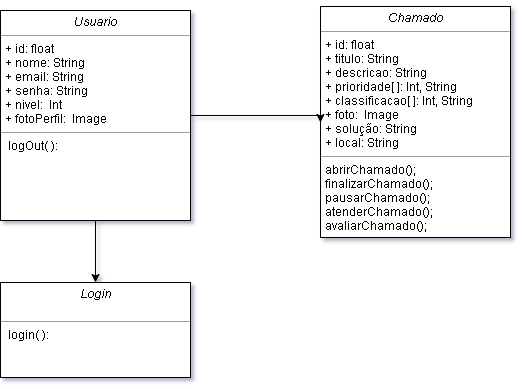
\includegraphics [scale = 0.83]{img/Diagramas/diagrama_classes.png}}
     \end{frame}
     \label{fig:diagrama_classes}
 \end{figure}
\newpage

\subsection{Resultados esperados}
Ao se atingir o prazo final para o fim do desenvolvimento, era esperado que o app desenvolvido proponha a capacidade de abrir chamados de suporte, acompanhar os chamados abertos e avaliar os chamados depois de atendidos, além de permitir que um usuário de nível atendente seja capaz de manipular o status de chamado entre "em espera", "em atendimento", "pausado" e "finalizado". O app deve rodar em smartphones com sistema operacional Android. 

Apesar de o aplicativo ser desenvolvido em uma plataforma de código híbrido, o uso em aparelhos com IOS só pode ser feito a partir do download da loja de aplicativos da Apple ou usando um computador com MacOS como ambiente de desenvolvimento, o que não se identifica como o cenário atual para desenvolvimento do aplicativo pelos acadêmicos, os mesmos somente possuem acesso a computadores com sistema operacional Windows e Linux, assim como somente smartphones Android. No entanto, devido aos fundamentos do framework Flutter, o mesmo projeto pode ser compilado em um computador com MacOS e com um aparelho IOS e funcionar da mesma maneira,  

\subsection{Áreas afetadas}
No ambiente da empresa, podem-ser afetadas principalmente a área de infraestrutura de TI, principalmente no quesito de organização das atividades do atendente. Além disso pode afetar todas as áreas da empresa que eventualmente façam pedidos para a área de infraestrutura de TI.

\section{Apresentação do aplicativo desenvolvido}
Esse capítulo aborda a apresentação do que foi desenvolvido como interface final do app. Assim como a apresentação do software em relatório, foi feita a documentação do app para o usuário, disponível no Apêndice III deste documento. 

De forma básica, o app baseia-se em uma tela principal com a visualização de 4 abas, sendo essas os status de um chamado. O protótipo do aplicativo também dispõe de uma tela de login que da acesso a tela dos chamados. 

A tela principal, além das 4 abas para mostrar os chamados em seus status, dá acesso a tela de criar chamado através do \textit{Floating Action Button} com o \textit{label} '+ Novo' e também um menu lateral como um \textit{Drawer} onde deve ser exibida as informações do usuário acessado. O login dos atendentes deve ser feito por um usuário e senha criados, até então, de forma manual através do Acesso ao Firebase, já para os demais usuários, o login deve ser a partir de uma conta google.

Também foi elaborado um resumo expandido com os resultados do trabalho para apresentações em futuros eventos. O resumo expandido pode ser encontrado no Apêndice IV deste documento.
\newpage
A Figura \ref{fig:1_login} representa a tela de login, na qual há os campos de usuário e senha com um botão para fazer o login. Ao clicar no botão de login, o app deve redirecionar para a página principal dos chamados.
\begin{figure}[htb]
     \caption{Print de tela 1 - Tela de login}
     \centering
     \begin{frame}{
     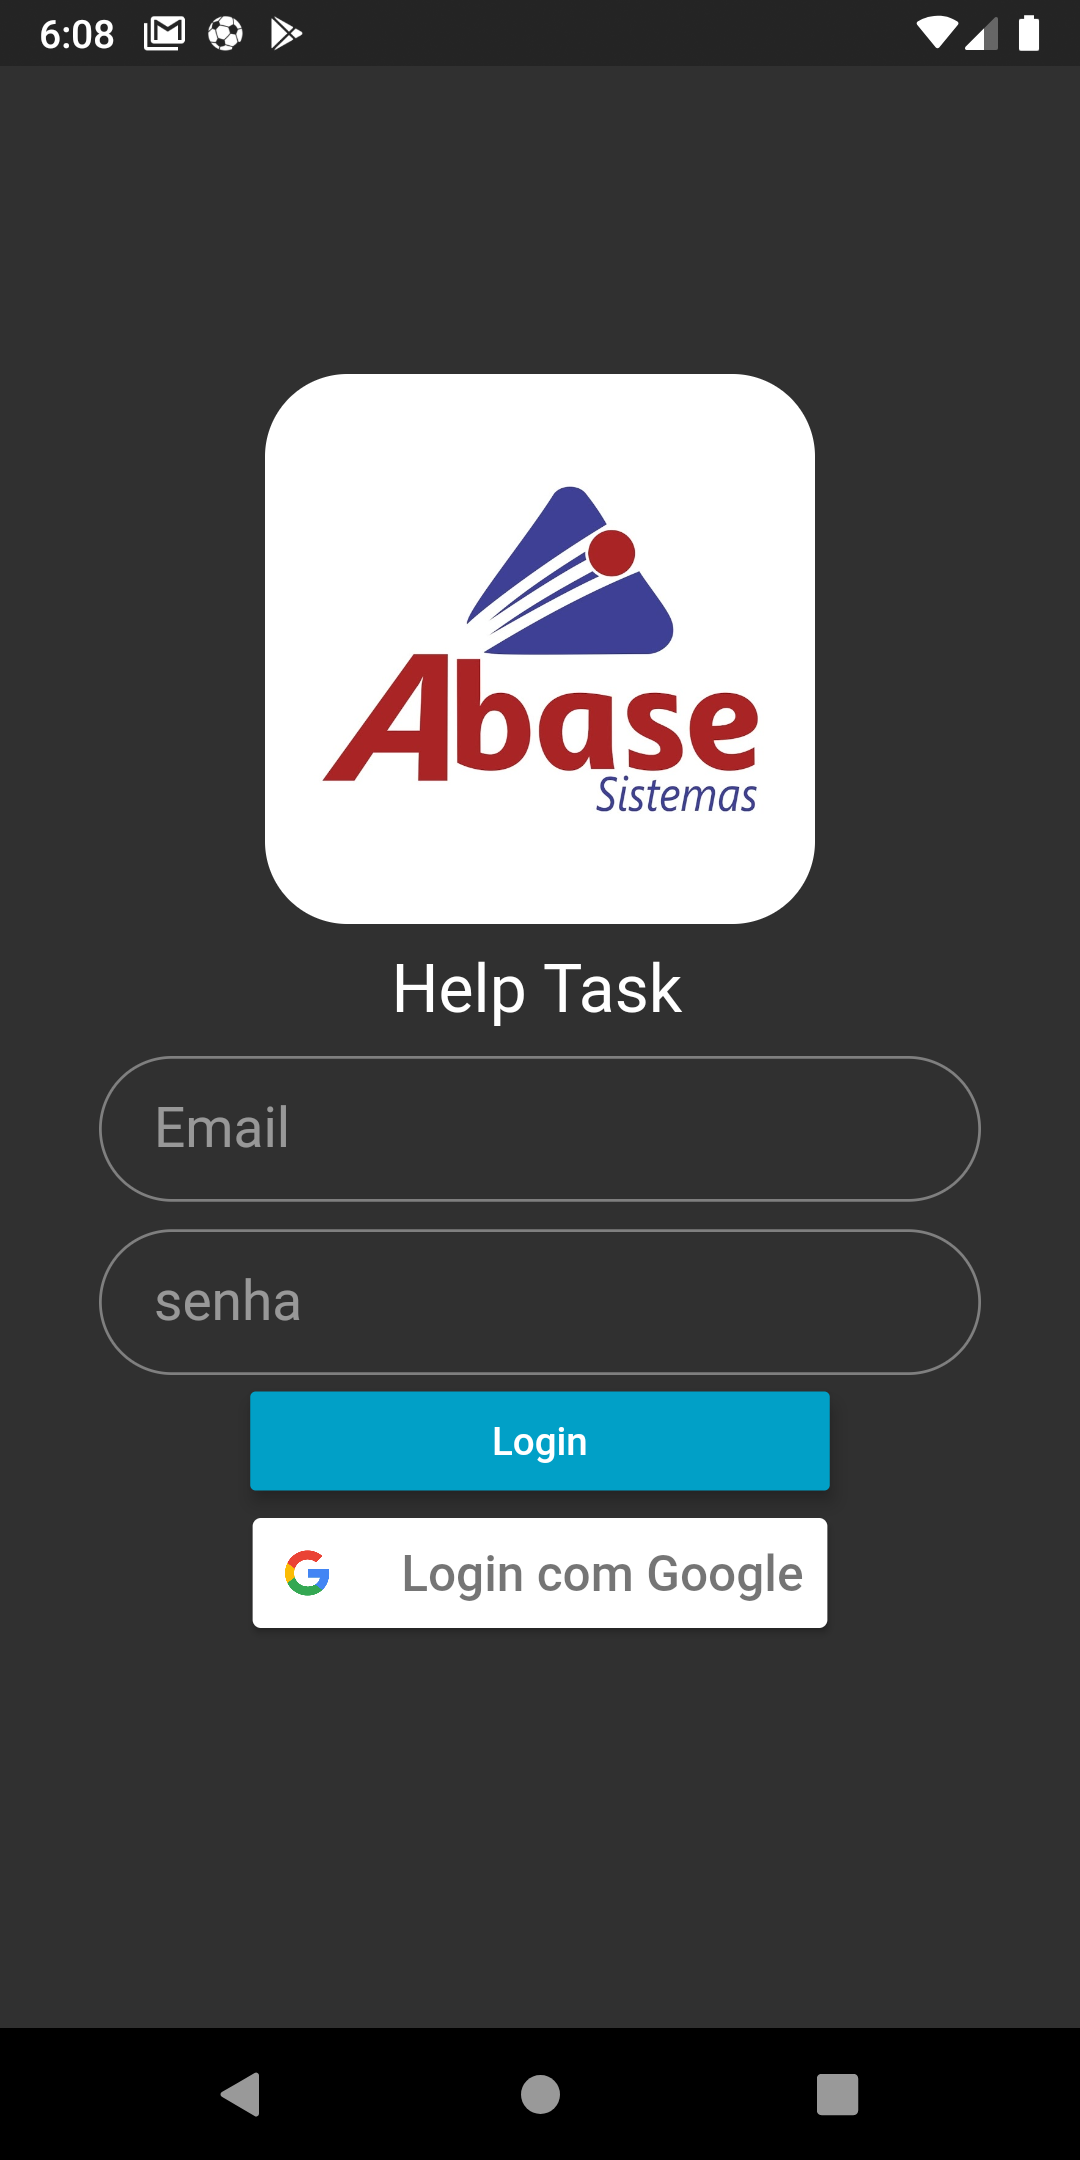
\includegraphics [scale = 0.2]{img/screenshots/1_login.png}}
     \end{frame}
     \label{fig:1_login}
 \end{figure}
\newpage

A Figura \ref{fig:2_em_espera} Representa a tela principal com a aba de chamados em espera, nessa tela são listados todos os chamados que ainda não foram atendidos, portanto os chamados podem ser atendidos ou finalizados diretamente.
\begin{figure}[htb]
     \caption{Print de tela 2 - Lista de chamados em espera}
     \centering
     \begin{frame}{
     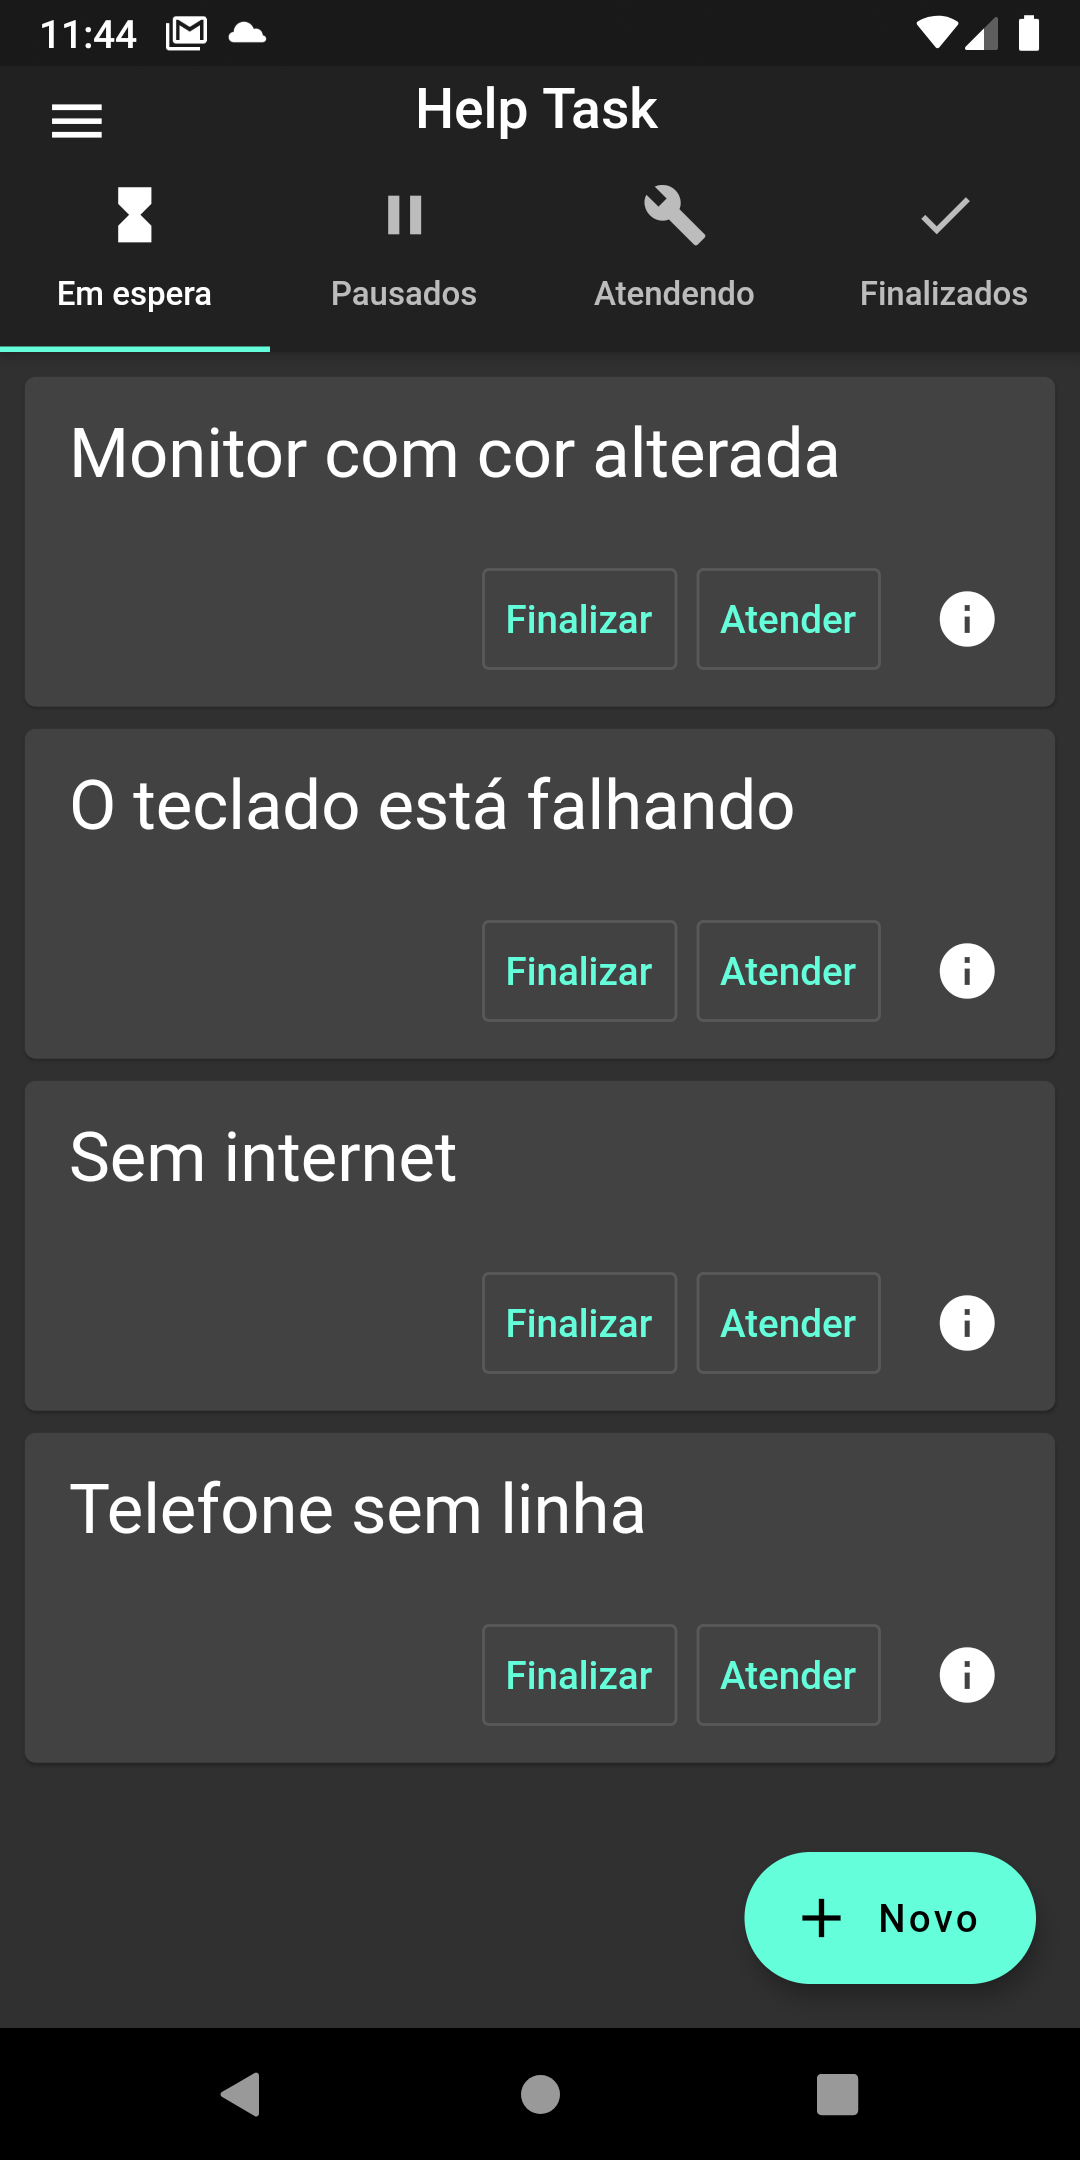
\includegraphics [scale = 0.2]{img/screenshots/2_em_espera.png}}
     \end{frame}
     \label{fig:2_em_espera}
 \end{figure}
\newpage

Na aba de chamados pausados, como mostra a Figura \ref{fig:3_pausados}, se localizam os chamados  que já foram atendidos pelo menos uma vez, nessa parte os chamados podem ser retomados para voltar a aba de atendimento.
\begin{figure}[htb]
     \caption{Print de tela 3 - Lista de chamados pausados}
     \centering
     \begin{frame}{
     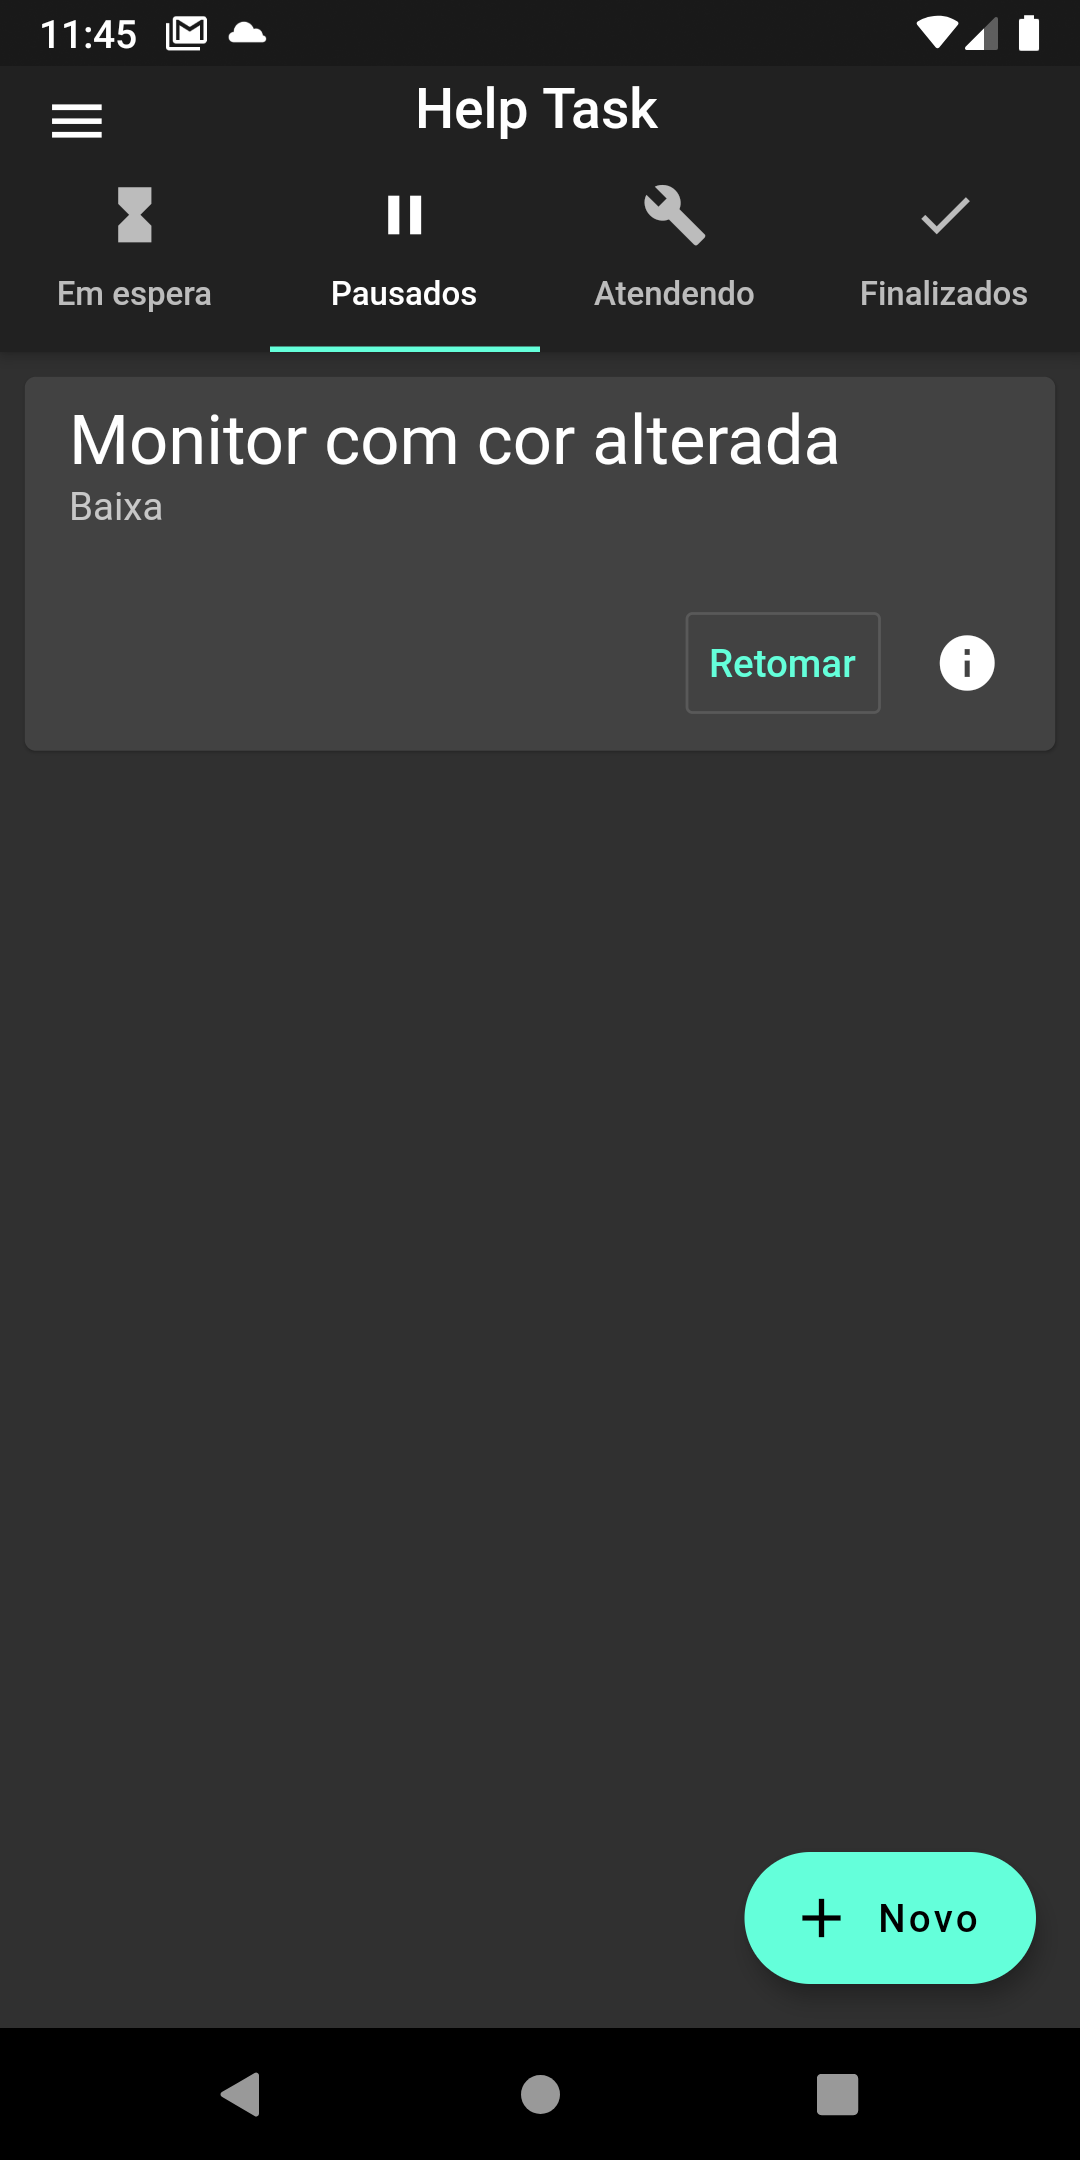
\includegraphics [scale = 0.2]{img/screenshots/3_pausados.png}}
     \end{frame}
     \label{fig:3_pausados}
 \end{figure}
\newpage

Na aba de chamados em atendimento, conforme a Figura \ref{fig:4_atendendo}, se localizam os chamados que estão sendo atendidos. Nessa parte, os chamados podem ser finalizados ou pausados. Para Finalizar um chamado o atendente deve informar uma justificativa.

\begin{figure}[htb]
     \caption{Print de tela 4 - Lista de chamados em atendimento}
     \centering
     \begin{frame}{
     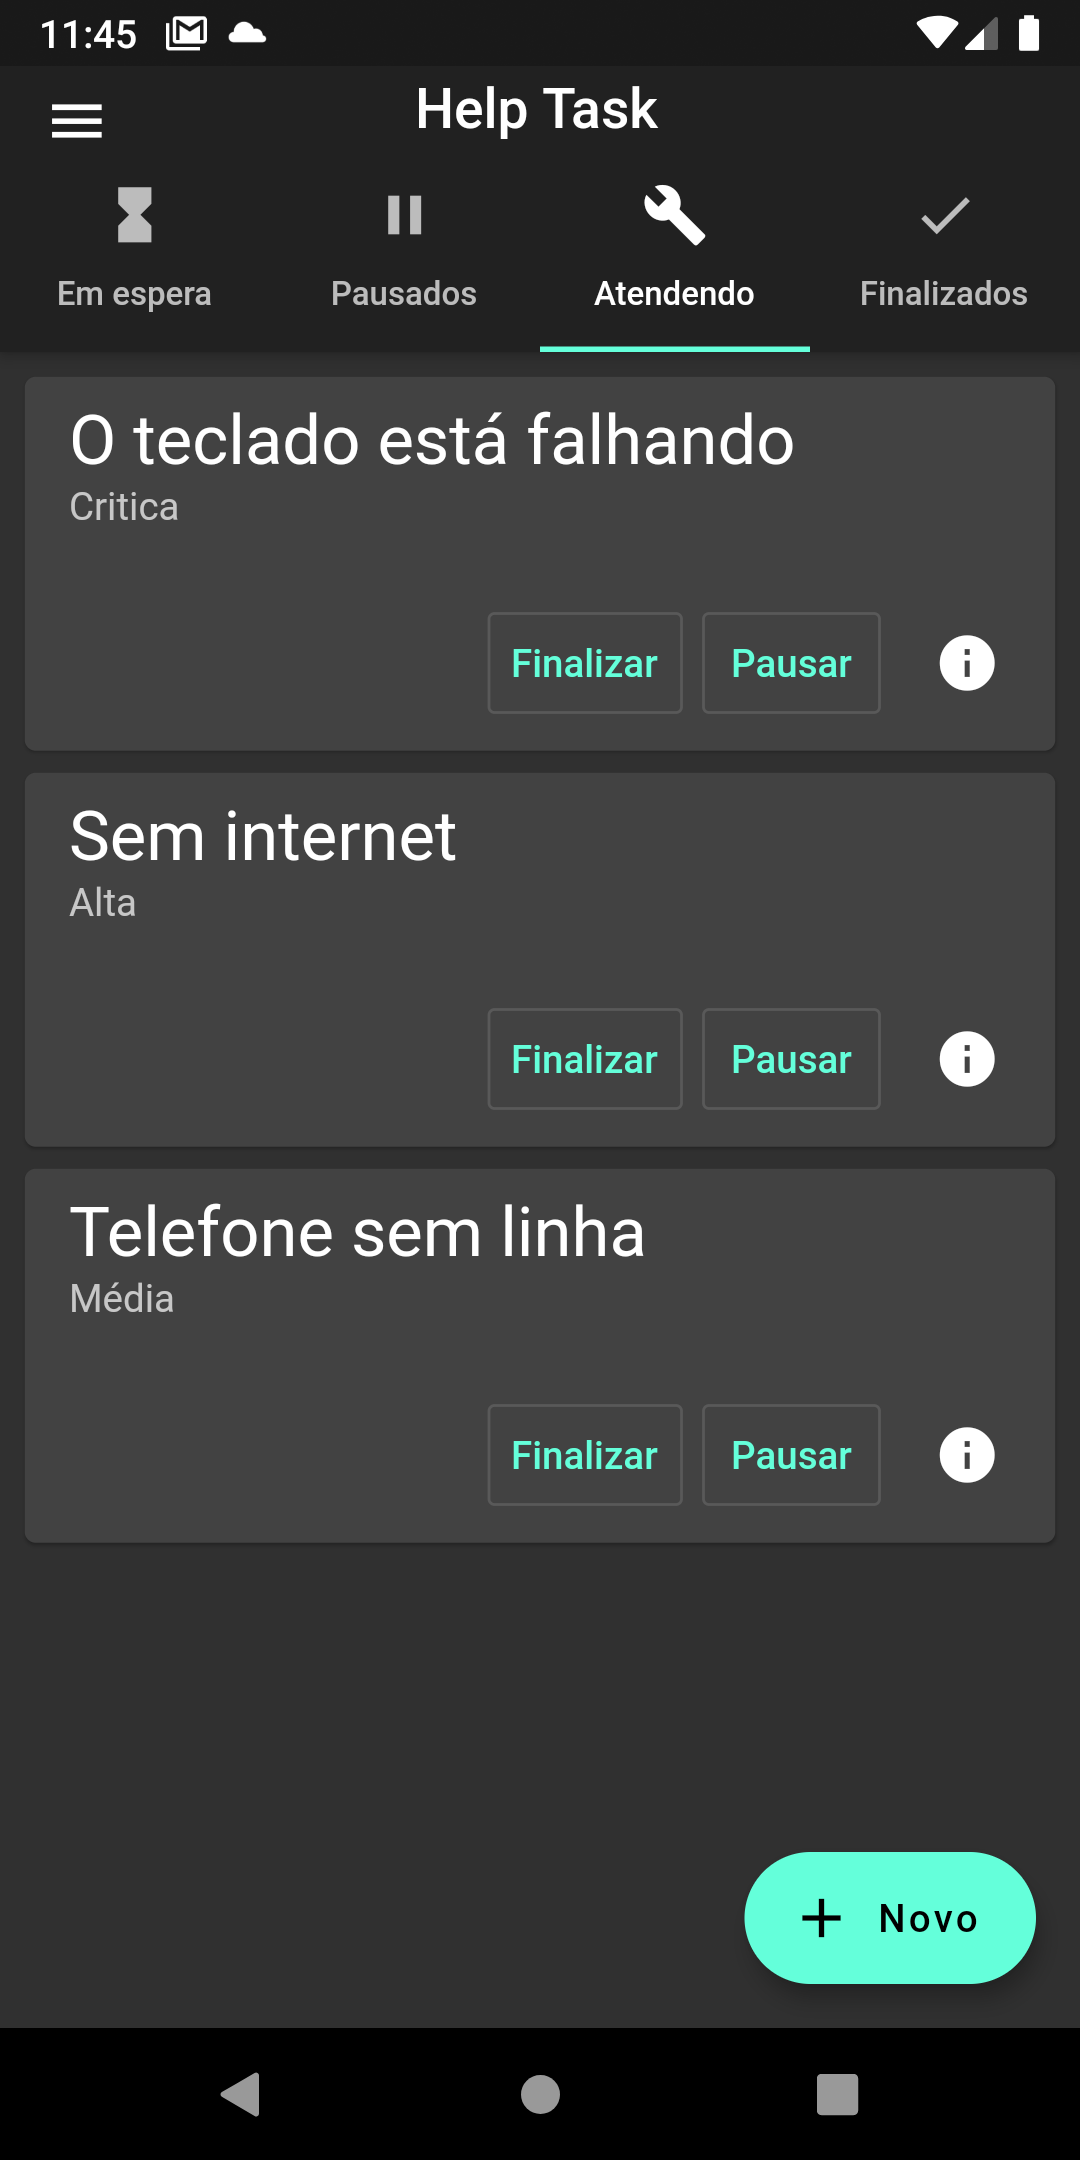
\includegraphics [scale = 0.2]{img/screenshots/4_atendendo.png}}
     \end{frame}
     \label{fig:4_atendendo}
 \end{figure}
\newpage

Na aba de chamados finalizados, conforme a Figura \ref{fig:5_finalizado}, se localizam os chamados que já foram atendidos e finalizados.
\begin{figure}[htb]
     \caption{Print de tela 5 - Lista de chamados finalizados}
     \centering
     \begin{frame}{
     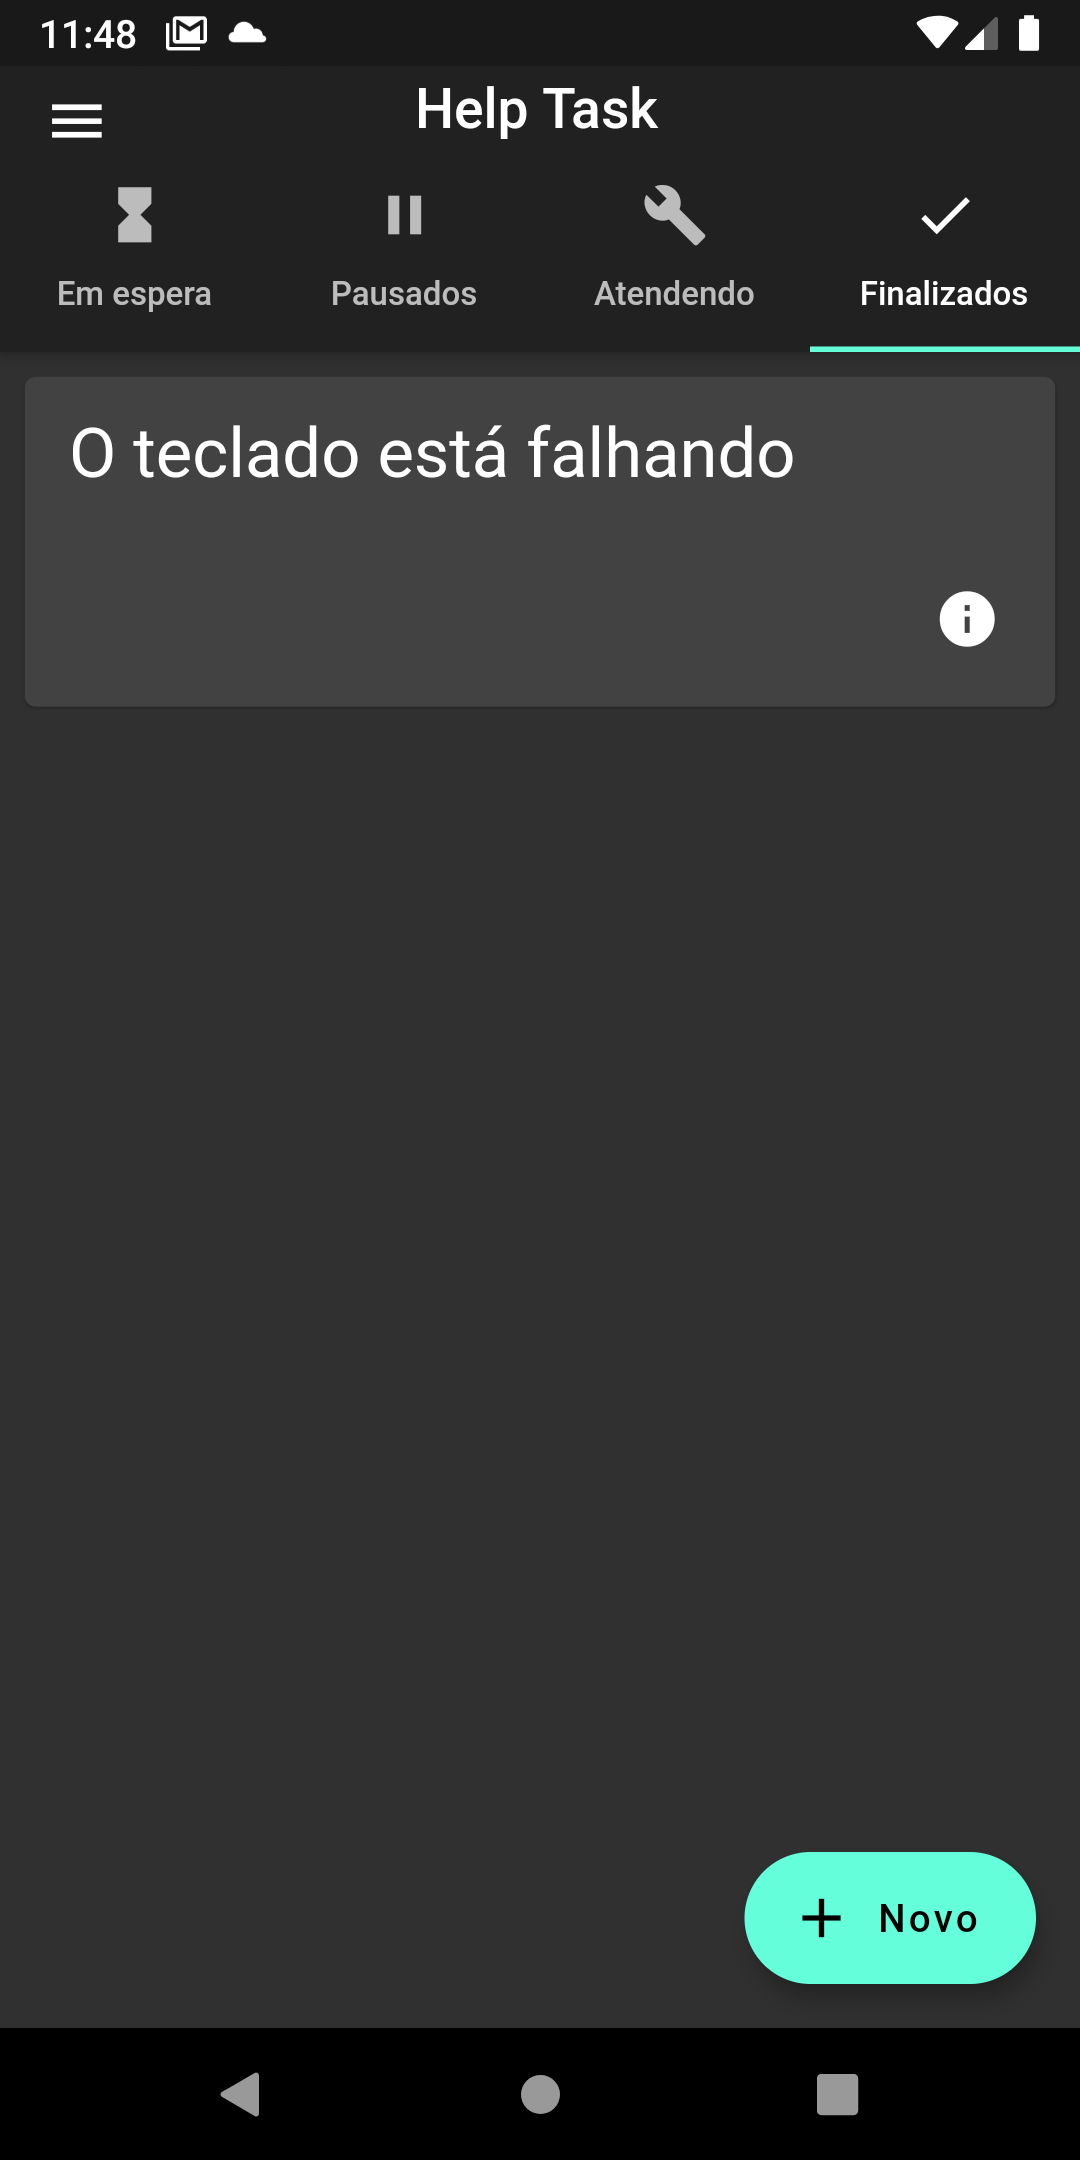
\includegraphics [scale = 0.2]{img/screenshots/5_finalizado.png}}
     \end{frame}
     \label{fig:5_finalizado}
 \end{figure}
\newpage

Em cada \textit{card} de chamado há um ícone de informações, localizado na parte inferior direita do mesmo. Esse ícone se clicado exibe as informações referentes a esse chamado, se os detalhes forem visualizados na tela de finalizados, serão exibidas todas as informações como classificação, tipo, descrição, momento de abertura e resolução. conforme a figura \ref{fig:detalhes}

\begin{figure}[htb]
     \caption{Print de tela 6 - Informações do chamado}
     \centering
     \begin{frame}{
     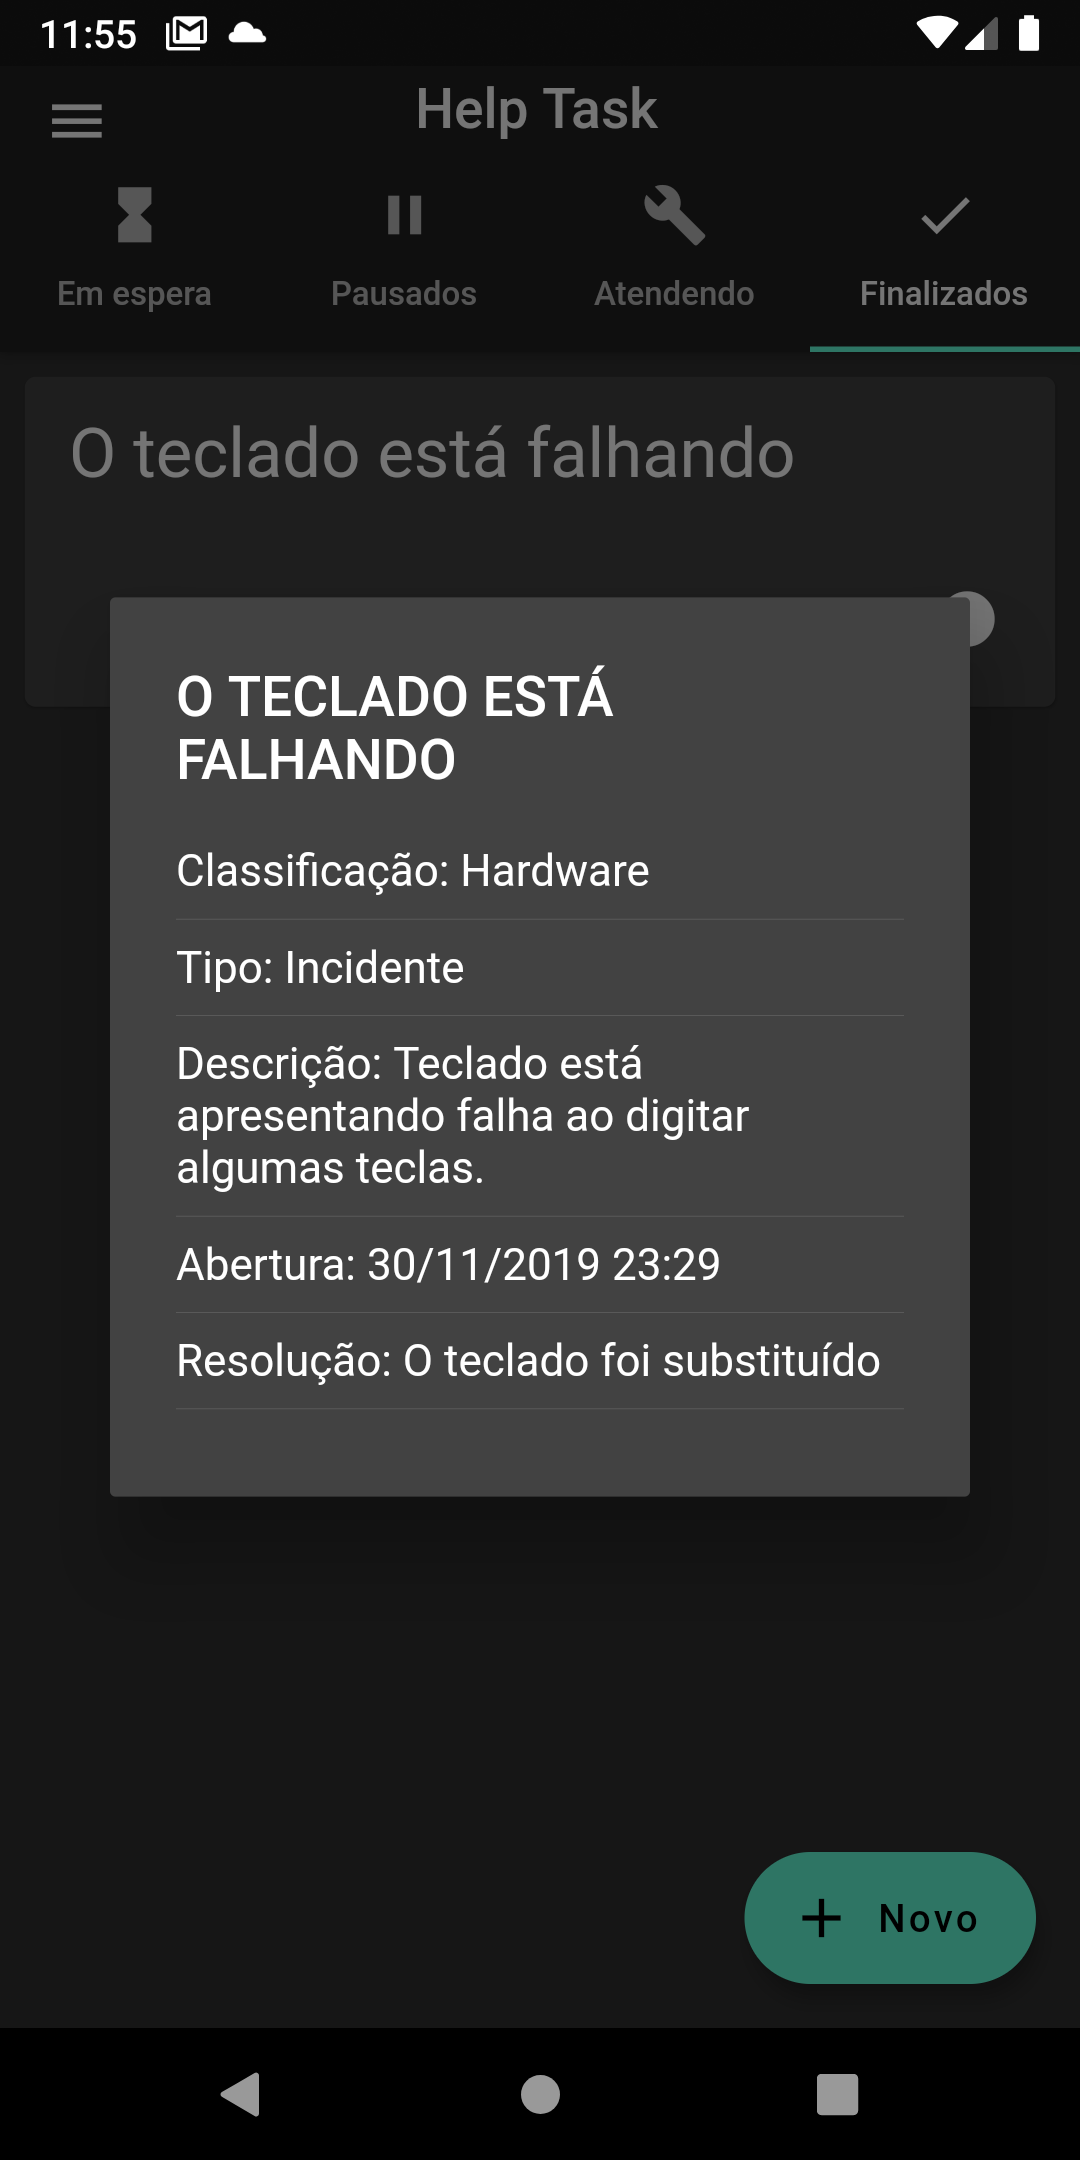
\includegraphics [scale = 0.2]{img/screenshots/detalhes.png}}
     \end{frame}
     \label{fig:detalhes}
 \end{figure}
\newpage


No menu lateral do app, localizam-se as informações do usuário logado como foto de perfil e e-mail. Também encontram-se os botões que levam até a tela de ajuda, onde se encontra uma visualização da documentação do app para o usuário, igual a presente no Apêndice C deste relatório. Também é possível acessar a tela de estatísticas, criar um novo usuário administrador ou fazer logout da sessão.
\begin{figure}[htb]
     \caption{Print de tela 7 - Menu lateral}
     \centering
     \begin{frame}{
     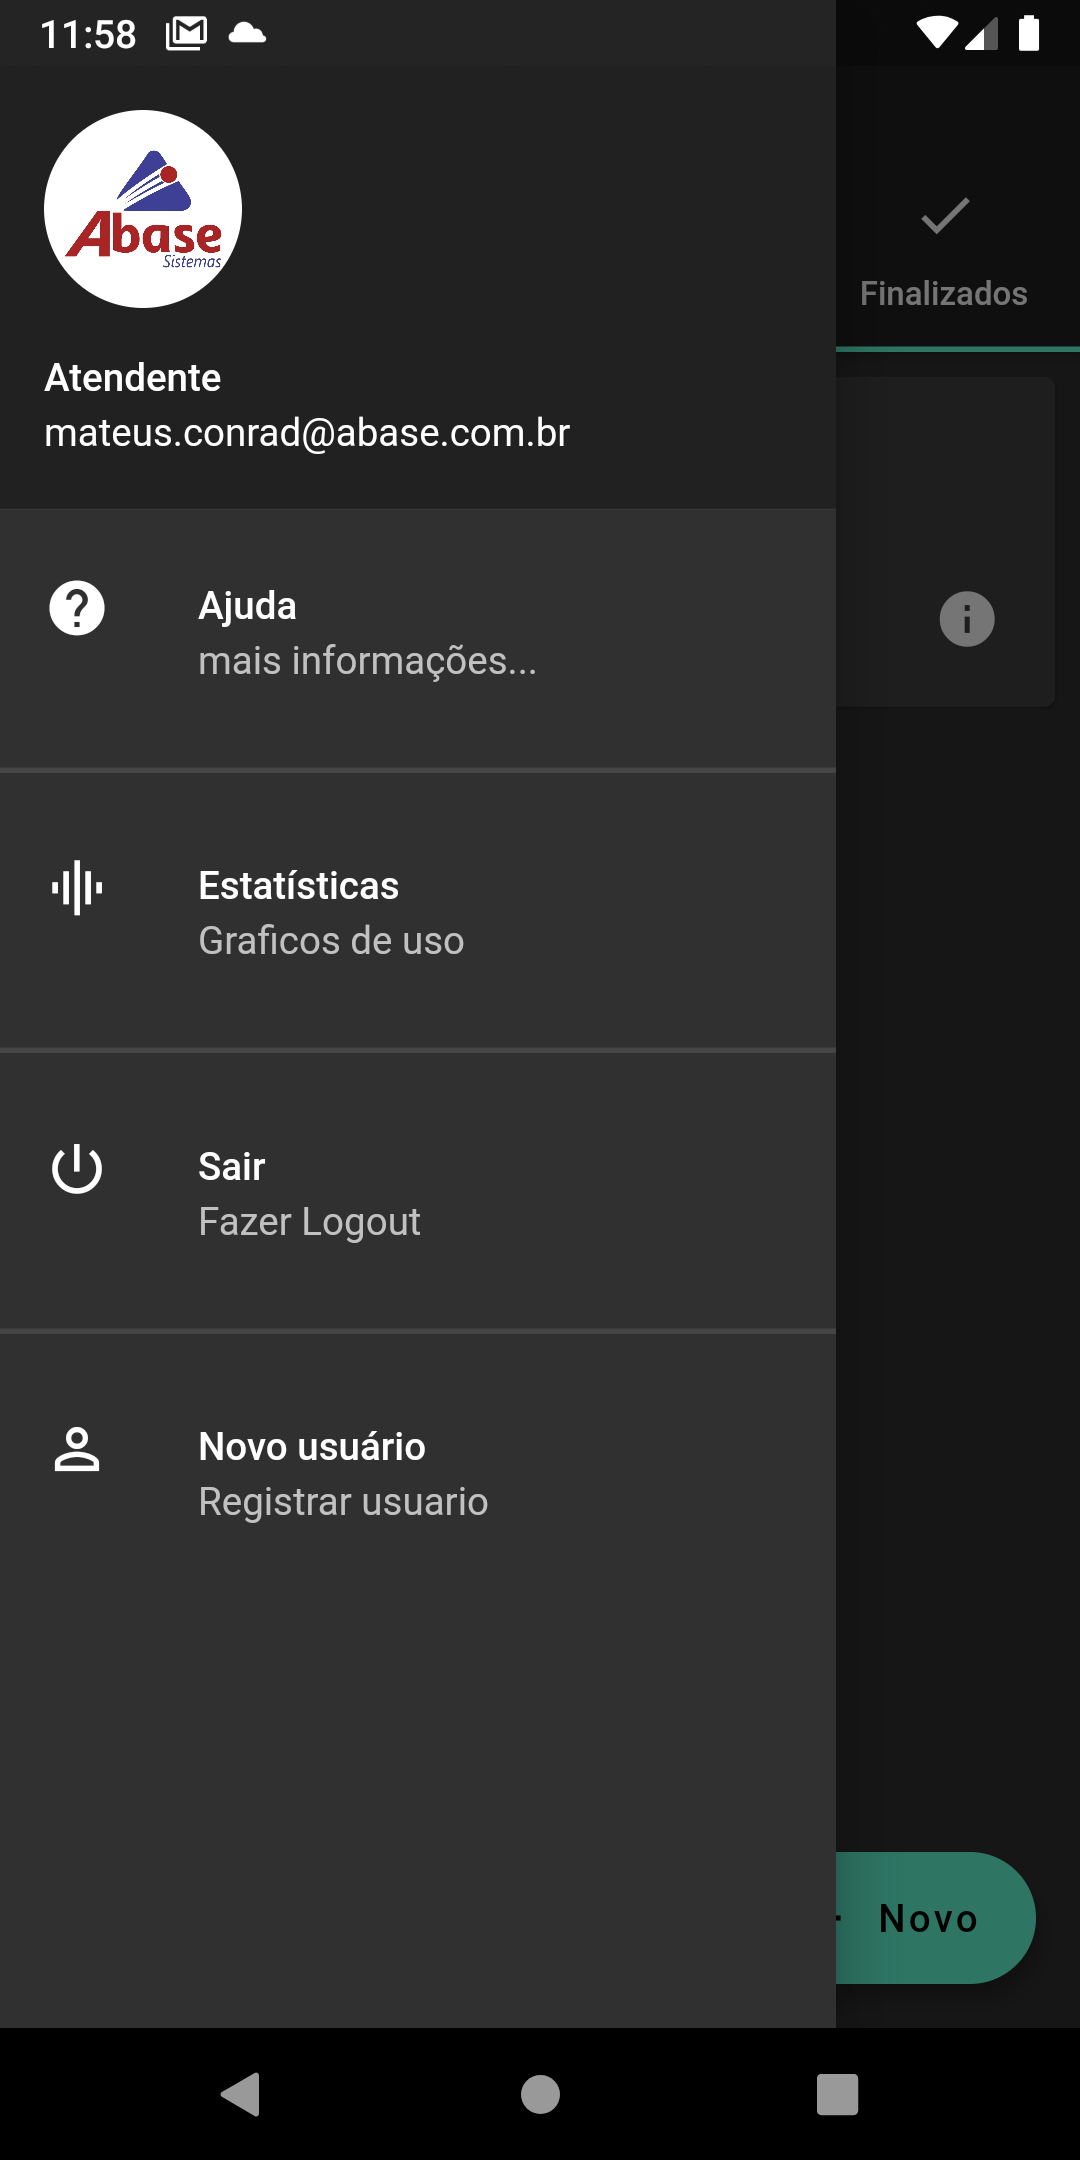
\includegraphics [scale = 0.2]{img/screenshots/6_drawer.png}}
     \end{frame}
     \label{fig:6_drawer}
 \end{figure}
 \newpage
 
 Na tela de abertura de chamado, acessada pelo \textit{Floating Action Button} presente na tela principal, permite colocar um título, descrição, prioridade, classificação e uma foto, conforme a descrição do RF1.
 \begin{figure}[htb]
     \caption{Print de tela 8 - Tela de abrir chammado}
     \centering
     \begin{frame}{
     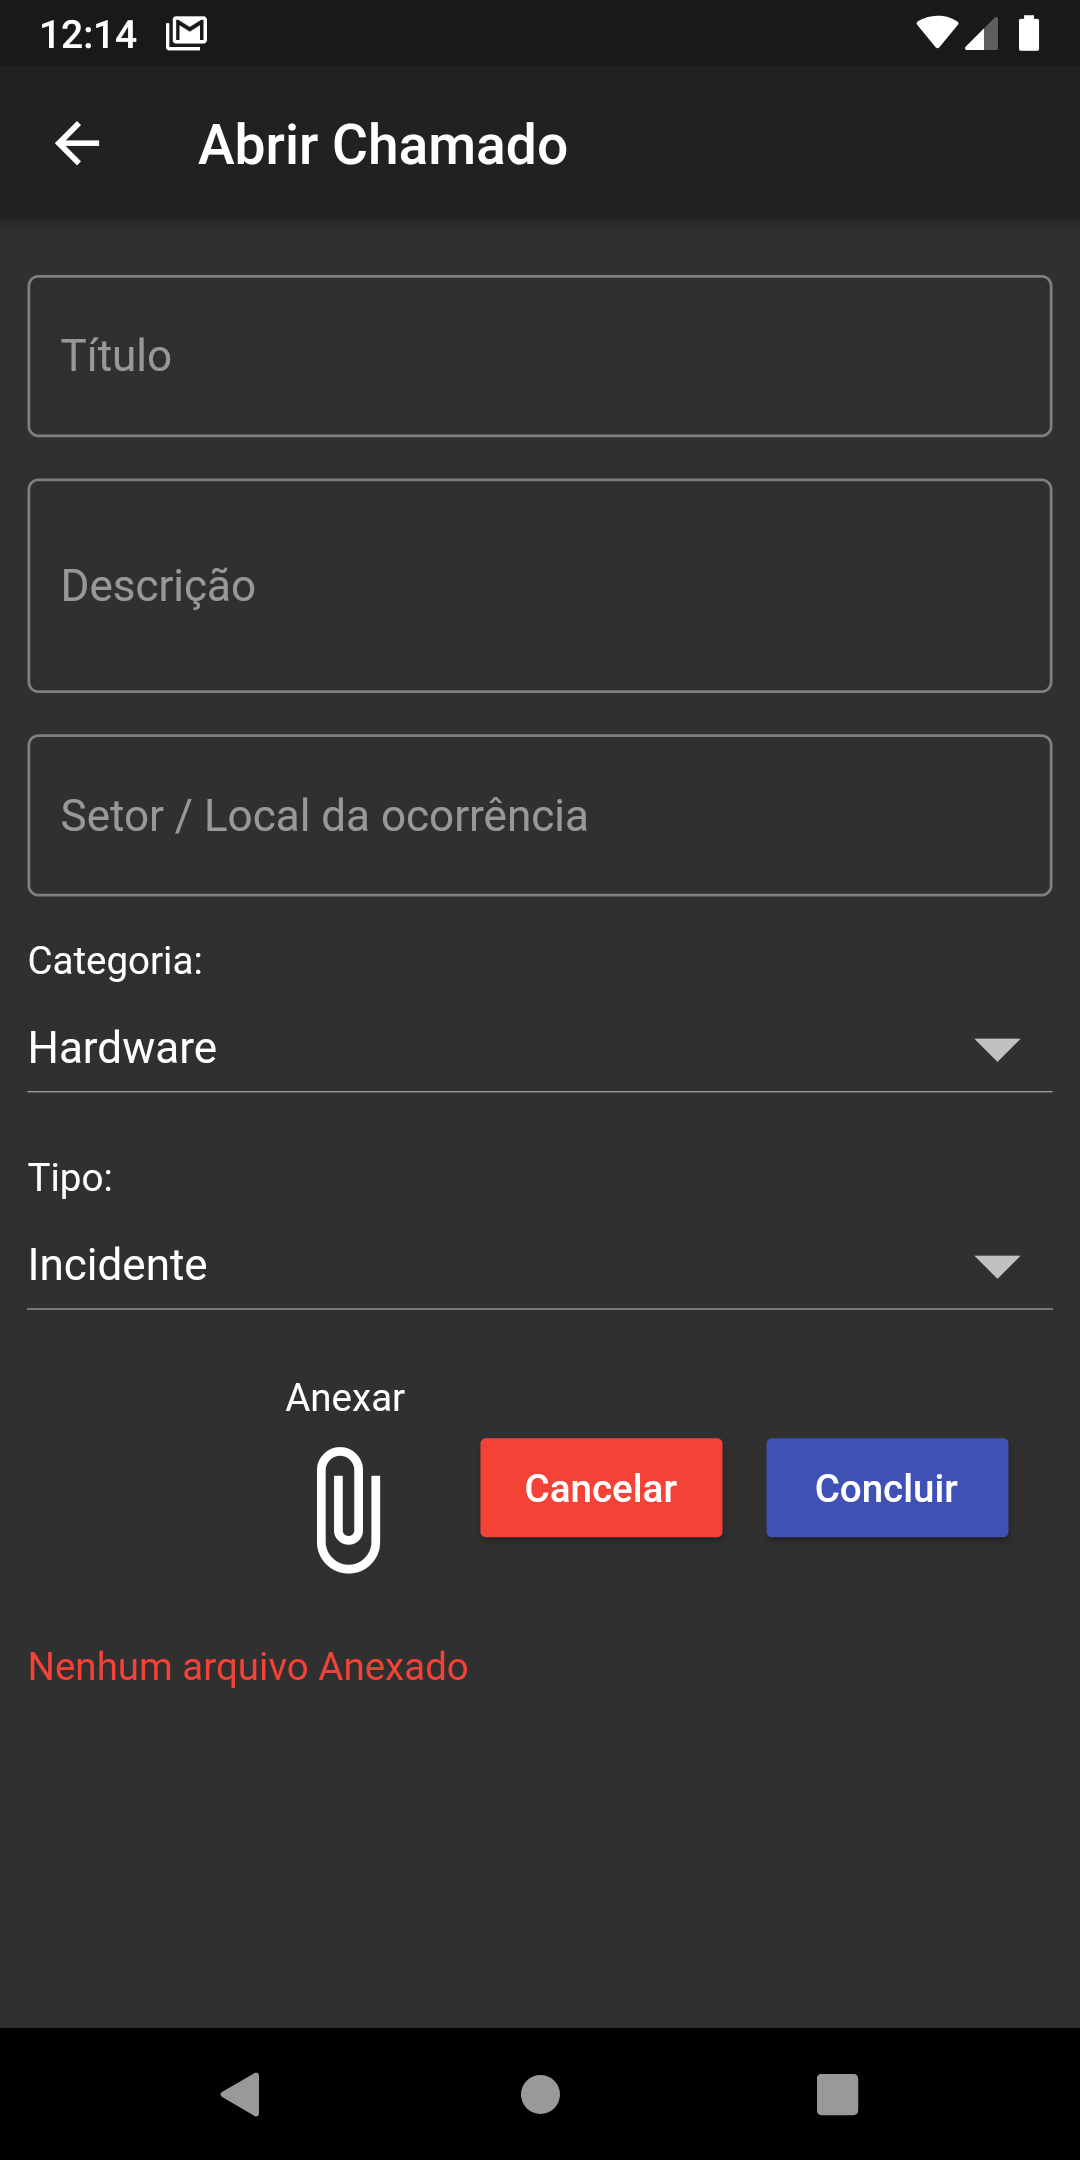
\includegraphics [scale = 0.2]{img/screenshots/7_abrir_chamado.png}}
     \end{frame}
     \label{fig:7_abrir_chamado}
 \end{figure}
 
 Na aba de chamados em espera, é possível atender o chamado ou finalizar o mesmo diretamente. Para atender o chamado é necessário informar uma prioridade, da mesma forma que ao finalizar o chamado é necessário descrever a resolução do mesmo.
\newpage

\section{Arquitetura de Desenvolvimento}
Devido a baixa complexidade tanto na estrutura proposta na análise do aplicativo como no desenvolvimento usando Flutter junto com o Firebase, não se fez necessário o uso de uma padronização de código, como por exemplo a MVC (\textit{Model, View and Controller}) onde o código é separado na parte de \textit{frontend}, operações de \textit{backend} e operações com banco de dados. Parte disso se deve ao não desenvolvimento de uma API, mas sim fazendo uso do Firebase como um \textit{BaaS} e \textit{Storage}.

Como organização do código, foi definido que a maneira mais simples de controlar a organização seria definir cada tela como uma classe dart e também na própria classe, criar métodos para simplificar o entendimento do código.

Como o método \textit{main()} apenas chama a classe \textit{Login()}, essa é a tela que será exibida ao abrir o aplicativo. Exemplificando, ainda usando a classe \textit{Login()} como exemplo, no código desta há a declaração da classe em si, que se dá por um \textit{Stateful Widget} e seu conteúdo dentro de um Widget chamado Scaffold, como pode ser observado no trecho de código 2. O Scaffold contém apenas chamadas para os métodos que exibem a imagem de logo, título do app e campos de login, esse mesmo estilo de programação foi usado em todo o código.
\begin{lstlisting}[numbers=left, language=Java, style=mycode, caption={Trecho de Código página de Login}, label={lst:loginpage-code}]
class Login extends StatefulWidget {
  @override
  _LoginState createState() => _LoginState();
}
class _LoginState extends State<Login> {
/*aqui se inclui todo o resto do codigo da classe, como declaracao de variaveis, metodos e os Widgets*/ 
}
\end{lstlisting}
\source{Adaptado do repositório do github.com/mateusconrad/app\_suporte}
\justifying\setlength{\parindent}{1,25cm} 

\newpage
Na figura \ref{fig:arquitetura_lib}, pode-se observar a estrutura de arquivos que compõem a pasta lib. Essa é a pasta padrão de um projeto flutter para os arquivos das classes. A pasta lib foi divida em outras três pastas e também contém 3 arquivos em sua raíz, sendo respectivamente as pastas "\textit{drawer}", "\textit{tabs}", "telas" e os arquivos \textit{home}, \textit{login} e \textit{main}.

 \begin{figure}[htb]
     \caption{Classes diretório Lib}
     \centering
     \begin{frame}{
     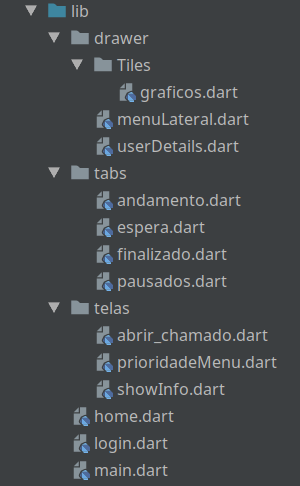
\includegraphics [scale = 0.8]{img/arquitetura_lib}}
     \end{frame}
     \label{fig:arquitetura_lib}
 \end{figure}

Começando pelos arquivos na raíz da pasta lib, há o arquivo main, que contém o método principal para inciar o aplicativo. O código contido no arquivo main faz uma chamada para abrir a tela de login, que dessa forma se identifica como a página principal do aplicativo, conforme o trecho de código 3.

\newpage

\begin{lstlisting}[numbers=left, language=Java, style=mycode, caption={Trecho de Código página do main()}, label={lst:main-code}]
void main() {
  runApp(MaterialApp(
    debugShowCheckedModeBanner: false,
    home: Login(), //chamada para pagina de login
  ));
}

\end{lstlisting}
\source{Adaptado do repositório do github.com/mateusconrad/app\_suporte}
\justifying\setlength{\parindent}{1,25cm} 

Quando o usuário é autenticado pela página de login, o mesmo é redirecionado para a página Home, identificada pelo arquivo \textit{home.dart} e por sua classe \textit{TabBarHome()}. O método de login com redirecionamento pode ser conferido no trecho de código 4.

\begin{lstlisting}[numbers=left, language=Java, style=mycode, caption={Trecho de Código do método de login}, label={lst:signin-code}]

final GoogleSignInAccount googleUser = await _googleSignIn.signIn();
final GoogleSignInAuthentication googleAuth = await googleUser.authentication;
final AuthCredential credential = GoogleAuthProvider.getCredential(
  accessToken: googleAuth.accessToken,
  idToken: googleAuth.idToken,);
FirebaseUser userDetails = (await _auth.signInWithCredential(credential));
ProviderDetails providerInfo = new ProviderDetails(userDetails.providerId);
List<ProviderDetails> providerData = new List<ProviderDetails>();
providerData.add(providerInfo);
UserDetails details = new UserDetails(userDetails.providerId, userDetails.displayName, userDetails.photoUrl,userDetails.email,providerData,);
final user = UserDetails;
Navigator.pushReplacement(context,
    new MaterialPageRoute(builder: (context) => new TabBarHome(),),);
    return userDetails;
  }
\end{lstlisting}
\source{Adaptado do repositório do github.com/mateusconrad/app\_suporte}
\justifying\setlength{\parindent}{1,25cm} 

\newpage
\section{Estrutura dos dados e autenticação}
No que diz respeito a estrutura de dados, foi usado a forma que o próprio Firebase disponibiliza, a de banco orientada a documentos, onde há níveis de hierarquia entre coleções, documentos e campos. A figura \ref{fig:firestore1} exibe como fica a estrutura dos dados gerados da abertura ate a finalização de um chamado, onde há a coleção de chamados, listando todos os ID's de todos os chamados cadastrados e também exibindo todos os campos do chamado selecionado.

    \begin{figure}[htb]
        \caption{Dados de um chamado}
        \centering
        \begin{frame}{
        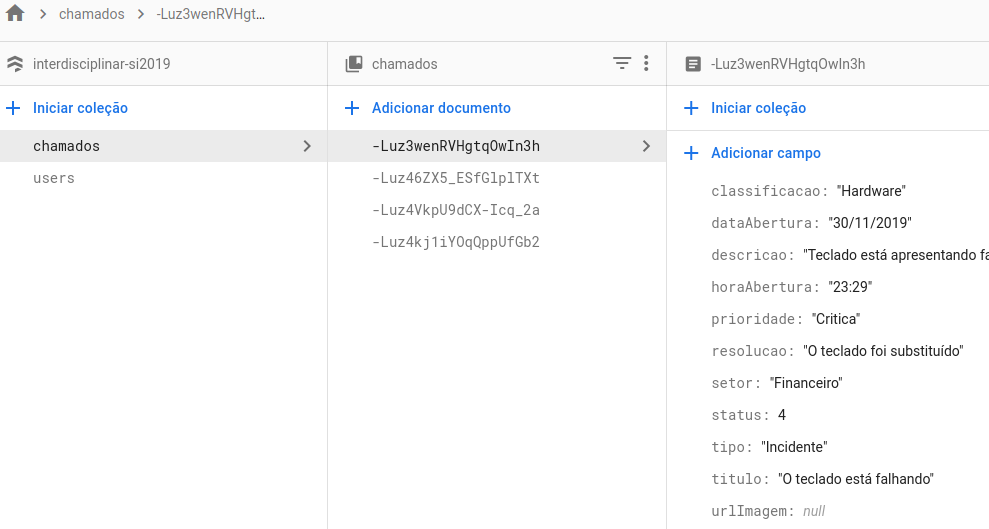
\includegraphics [scale = 0.44]{img/firestore1.png}}
        \end{frame}
        \label{fig:firestore1}
    \end{figure}

Assim como os chamados, os dados dos atendentes ficam registrados em banco. Os dados dos usuários são capturados através do método de \textit{Authentication} do firebase, onde foram habilitados os provedores de email e também o do google.   
    
    \begin{figure}[htb]
        \caption{Firebase Authentication}
        \centering
        \begin{frame}{
        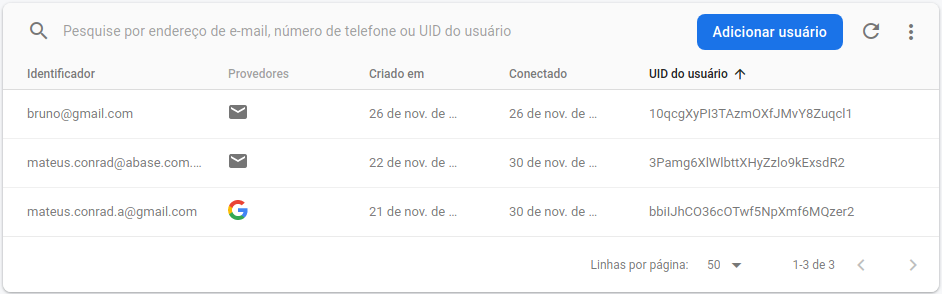
\includegraphics [scale = 0.455]{img/firestore2.png}}
        \end{frame}
        \label{fig:firestore2}
    \end{figure}


\section{Testes e Qualidade de Software}
Não foi aplicado nenhum tipo de teste de software como testes de unidade ou testes com usuários como o BDD( Behaviour Driven Development). Esses testes não foram aplicados devido a falta de tempo hábil para implantação e realização dos mesmos. No entanto ao pesquisar como testes de software podem ser realziados em apps desenvolvidos usando o flutter, chegou-se a informação que o framework em si possui suporte para três tipos de teste, sendo esses: Testes de unidade, teste de \textit{widgets} e teste de integração.
 
De acordo com a documentação do Flutter, os testes de unidade se propõem a testar partes isoladas do código, como funções métodos ou uma classe. Enquanto isso, os testes de Widget tem por função testar um único widget, em outros frameworks esse teste pode ser encontrado pelo nome de teste de componente. Por último, apresenta-se o teste de integração, que possui a tarefa de testar o aplicativo como um todo, ou em casos de aplicações muito grandes, isolar uma parte significativa do aplicativo e testá-la por completo.

A forma que o grupo encontrou de manter um controle sobre erros achados durante o desenvolvimento foi fazer o cadastro de \textit{issues} no repositório do código no github, assim cria-se uma linha de orientação ao momento de desenvolver. As issues funcionam como um cadastro de erros, problemas e melhorias a serem feitas no código. Todas as issues cadastradas que foram abertas ou fechadas podem ser verificadas em: <https://github.com/mateusconrad/app\_suporte/issues>, conforme a figura \ref{fig:issues_github}.
    
 \begin{figure}[htb]
     \caption{Issues Github}
     \centering
     \begin{frame}{
     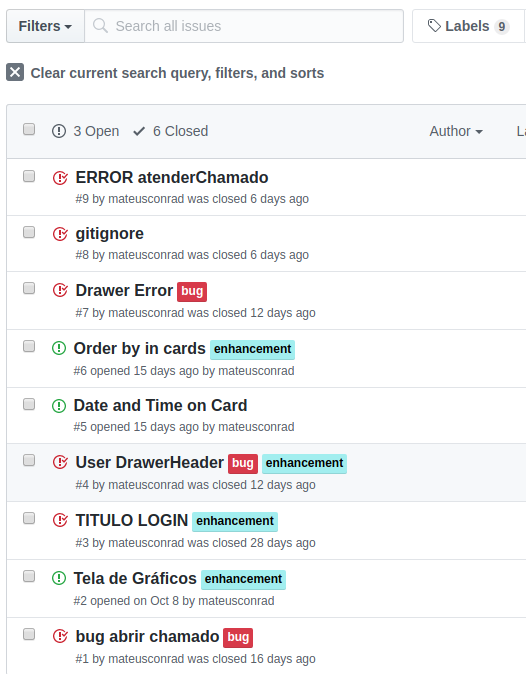
\includegraphics [scale = 0.6]{img/issues_github}}
     \end{frame}
     \label{fig:issues_github}
 \end{figure}
    